\documentclass[10pt,a4paper]{article}
\usepackage[utf8]{inputenc}
\usepackage[spanish]{babel}
\usepackage[margin=1in]{geometry}
\usepackage{amsmath}
\usepackage{amsfonts}
\usepackage{amssymb}
\usepackage{enumitem}
\usepackage{hyperref} 
\usepackage{graphicx}
\usepackage{url}
\usepackage{breakurl}
\hypersetup{pdftex,colorlinks=true,allcolors=black}
\hypersetup{
    pdftitle={},
    pdfauthor={Pablo Riutort Grande},
    pdfsubject={},
    bookmarksnumbered=true,     
    bookmarksopen=true,         
    bookmarksopenlevel=1,       
    colorlinks=true,            
    pdfstartview=Fit,           
    pdfpagemode=UseOutlines,    % this is the option you were lookin for
    pdfpagelayout=TwoPageRight
}
\usepackage{listings}
\usepackage{xcolor}
\usepackage{hypcap}
\definecolor{codegreen}{rgb}{0,0.6,0}
\definecolor{codegray}{rgb}{0.5,0.5,0.5}
\definecolor{codepurple}{rgb}{0.58,0,0.82}
\definecolor{backcolour}{rgb}{0.95,0.95,0.92}
\lstdefinestyle{mystyle}{
    backgroundcolor=\color{backcolour},   
    commentstyle=\color{codegreen},
    keywordstyle=\color{magenta},
    numberstyle=\tiny\color{codegray},
    stringstyle=\color{codepurple},
    basicstyle=\ttfamily\footnotesize,
    breakatwhitespace=false,         
    breaklines=true,                 
    captionpos=b,                    
    keepspaces=true,                 
    numbers=left,                    
    numbersep=5pt,                  
    showspaces=false,                
    showstringspaces=false,
    showtabs=false,                  
    tabsize=2
}
\lstset{style=mystyle}
\usepackage{xparse}
\usepackage{verbatim}
\NewDocumentCommand{\codeword}{v}{%
\texttt{{#1}}
}
\author{Pablo Riutort Grande}
\title{
	Seguridad del software\\
	\vspace{0.5cm}
	PEC 2\\
	\vspace{1cm}
	\textbf{Vulnerabilidades en software}
	\vspace{1cm}\\UOC - MISTIC
}



\begin{document}
\maketitle
\pagebreak
\tableofcontents
\lstlistoflistings
\listoffigures

\pagebreak

\section{}
\begin{comment}
Enunciado:
1) Funciones vulnerables (50%)

Realiza un programa sencillo en el cual se utilice una función vulnerable. 

Muestra y razona la vulnerabilidad en tiempo de ejecución de la función que has elegido y explica cómo y por qué la función es vulnerable.
\end{comment}

Para este ejercicio se ha elegido la función strcpy(). strcpy() copia el string dado por puntero a una localización destino [Ver \cite{strcpy}]. Esta función no verifica el tamaño de los buffers y puede sobreescribir zonas contiguas de memoria [Ver \cite{strcpy2}].

Se demostrará la vulnerabilidad haciendo una demostración con de un heap overflow [Ver \cite{heap}]. Esta vulnerabilidad de la familia del buffer overflow [Ver \cite{buffer}] consiste en sobreescribir la memoria heap , concretamente el instruction pointer. El heap es la porción de memoria donde la memoria alojada dinámicamente reside, típicamente con funciones como malloc se puede reservar memoria en ese segmento [Ver \cite{malloc}].\\

En el programa heap.c [Ver \ref{lst:heap}] tenemos 2 funciones: regular() es la función a la que se llegará en una ejecución normal de código y secret() es inaccesible.

Si ejecutamos el programa con parámetros normales llegamos a la función regular()
\lstinputlisting[
	language=C, 
	firstline=16, lastline=22,
	caption={[heap.c: regular() y secret()]{Funciones regular() y secret()}}
]{heap.c}

En el heap tendremos los siguientes objetos de manera consecutiva:

\lstinputlisting[
	language=C, 
	firstline=8, lastline=14,
	caption={[heap.c: Objetos en el heap]{Objetos en el heap}}
]{heap.c}

Con malloc reservamos el espacio en el memoria dinámica y se asigna por defecto la función regular():
\lstinputlisting[
	language=C, 
	firstline=28, lastline=36,
	caption={[heap.c: selector()]{Se asigna regular al selector de funciones}}
]{heap.c}

A continuación haremos un estudio del funcionamiento del heap introduciendo valores y viendo cómo se almacenan dichos valores en la memoria. Para eso ejecutaremos el programa con el debugger de gdb y exploraremos el contenido de la memoria a medida que los vamos ejecutando.\\

Primero situaremos un breakpoint antes de la finalización del programa y lo ejecutaremos con un input sencillo.  Una vez hecho esto, la memoria dinámica habrá sido creada por malloc y debería aparecer en el mapa del proceso que se está ejecutando, en nuestro caso podemos ver que empieza en la dirección 0x804d000 [Fig. \ref{fig:figura1}].

\begin{figure}[h!]
  \centering
  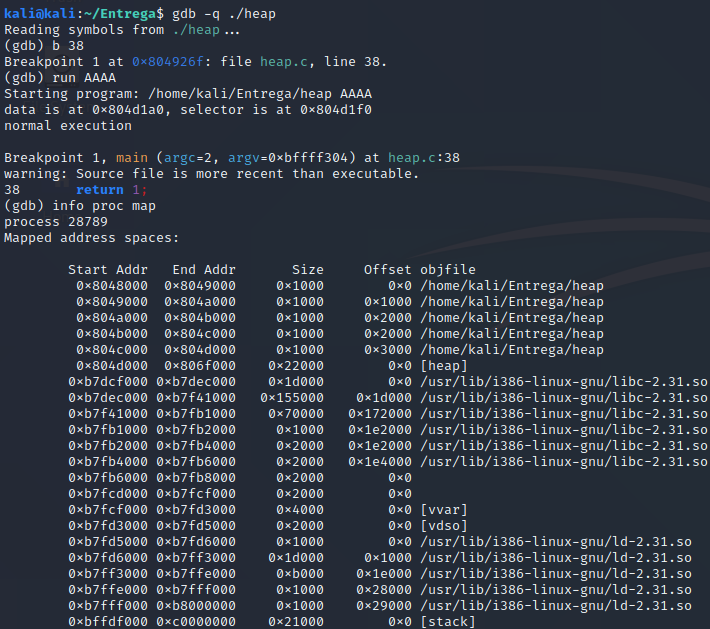
\includegraphics[scale=0.6]{1.png}\\
  \caption{Información del proceso ejecutándose}
  \label{fig:figura1}
\end{figure}

\pagebreak

Si inspeccionamos la memoria en la dirección donde empieza el heap podemos ver el contenido de los registros y concretamente cómo queda registrado nuestro input ``AAAA'' [Fig. \ref{fig:figura2}, Fig. \ref{fig:figura3}]. Otro dato importante es la dirección de memoria de regular(), es decir, la siguiente función a ejecutar 0x080491bd [Fig. \ref{fig:figura4}].
\begin{figure}[h!]
  \centering
  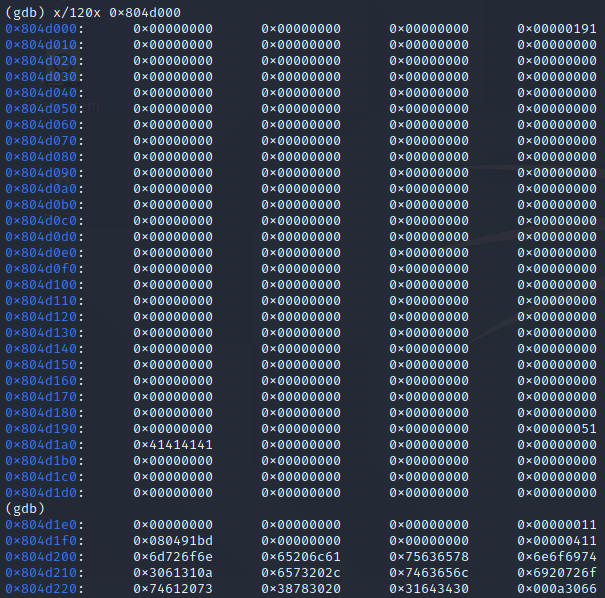
\includegraphics[scale=0.5]{2.png}\\
  \caption{Sección de memoria del heap}
  \label{fig:figura2}
\end{figure}

\begin{figure}[h!]
  \centering
  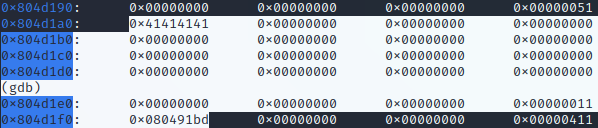
\includegraphics[scale=0.5]{2.1.png}\\
  \caption{Contenido de la memoria heap. Queda registrado nuestro input ``AAAA'' y la dirección de memoria de la siguiente función a ejecutar}
  \label{fig:figura3}
\end{figure}

\begin{figure}[h!]
  \centering
  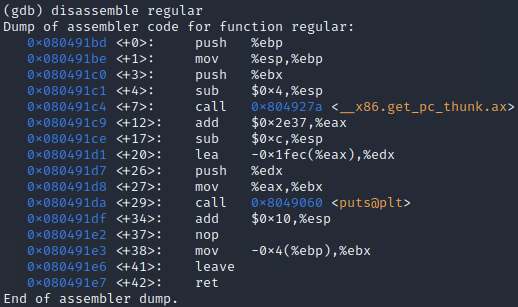
\includegraphics[scale=0.5]{3.1.png}\\
  \caption{Desensamblado de la función regular. Se sitúa en la dirección de memoria 0x080491bd}
  \label{fig:figura4}
\end{figure}

\pagebreak

Probamos una nueva ejecución con distinto input, esta vez vamos a probar con 90 caracteres ``A'' y observaremos  que el programa sufre un \textit{Segmentation fault} porque el registro de EIP (Instruction Pointer) tiene como contenido 0x41414141, es decir ``AAAA'' [Fig. \ref{fig:figura5}]. De esta forma ya sabemos cómo podemos modificar el registro EIP y ejecutar istrucciones arbitrarias, solo tenemos que modificar el input.
\begin{figure}[h!]
  \centering
  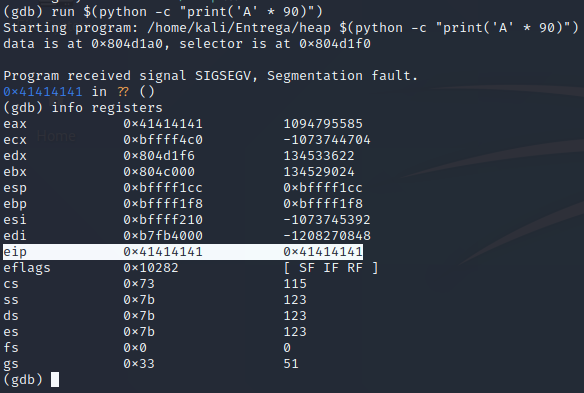
\includegraphics[scale=0.5]{4.png}\\
  \caption{Contenido del registro EIP}
  \label{fig:figura5}
\end{figure}

Iremos haciendo sucesivas pruebas hasta dar con el número adecuado de caracteres para que en el registro EIP se posicione lo que deseemos. La idea es identificar el número de caracteres necesarios para que los últimos coincidan exactamente con el registro EIP. En la figura [Fig. \ref{fig:figura6}] vemos que los caracteres ``BCDE'' quedan representados en el registro EIP, hemos dado con la forma de inyectar la dirección de memoria sustituyendo el  ``BCDE'' por la dirección de memoria deseada.
\begin{figure}[h!]
  \centering
  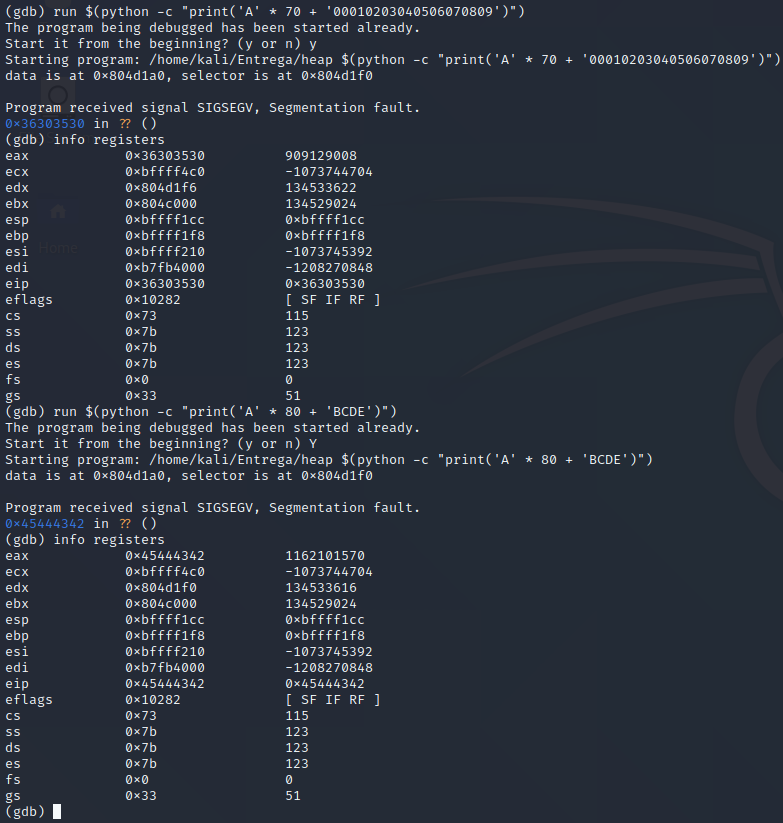
\includegraphics[scale=0.4]{5.png}\\
  \caption{Sucesivas pruebas con distintos caracteres.}
  \label{fig:figura6}
\end{figure}

\pagebreak

El input que sustituye a ``BCDE'' será el correspondiente a la dirección de memoria de secret [Fig. \ref{fig:figura7}]: 0x08049192. Para inyectar ese valor en hexadecimal recordemos que hay que construirlo de derecha a izquierda, entonces quedará un string tal que así: ``\textbackslash x92\textbackslash x91\textbackslash x04\textbackslash x08'' [Fig. \ref{fig:figura8}].
\begin{figure}[h!]
  \centering
  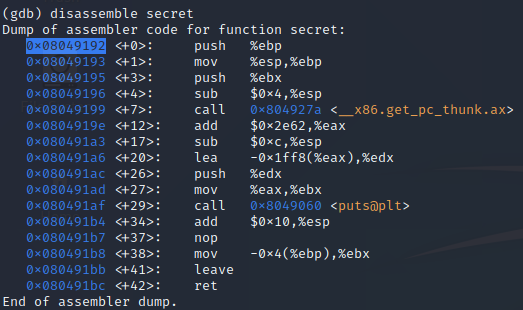
\includegraphics[scale=0.6]{3.png}\\
  \caption{La función secret tiene como dirección memoria la 0x08049192}
  \label{fig:figura7}
\end{figure}

\begin{figure}[h!]
  \centering
  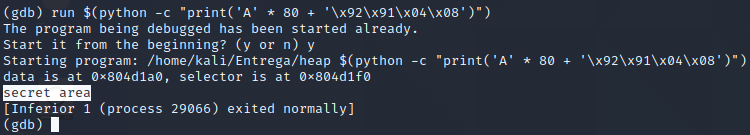
\includegraphics[scale=0.5]{6.png}\\
  \caption{Modifación exitosa del heap, hemos accedido a la función secreta}
  \label{fig:figura8}
\end{figure}


\pagebreak
\section{}
\begin{comment}
2) Vulnerabilidades Format String vs Stack overflow (50%)

¿En qué consisten las vulnerabilidades de tipo Format String?

¿Cómo puede ser explotado un Format String Bug?

¿Qué similitud y / o diferencia tiene respecto del stack overflow?

Realiza un programa sencillo donde se produzca la vulnerabilidad tipo Format String y muestra cómo se produce la vulnerabilidad en el momento de la ejecución.

Formato 

En el documento de desarrollo de la PEC es necesario aportar el código fuente de los programas, mostrar como se han producido la vulnerabilidades así como los valores de la pila (stack) utilizando herramientas como IDA, Immunity Debugger, OllyDbg o equivalente, también se deben aportar impresiones de pantalla de todo el proceso y razonar los pasos realizados así como las decisiones tomadas.

Los ejercicios se pueden realizar en un entorno Windows, Linux o Android

Formato de la entrega: Documento PDF y ficheros de código fuente.
\end{comment}
En C existen funciones especiales que se utilizan para representar tipos de datos por pantalla mediante una representación en string, estas funciones son las llamadas \textit{format functions}.\\
Estas funciones toman un número variable de argumentos, uno de ellos es el string de formato (\%) y mientras la función evalua este parámetro también accede a los parámetros extra añadidos. Su uso es muy útil para mostrar información variada por pantalla como mensajes o errores [Ver \cite{format2}].\\

\lstinputlisting[
	language=C, 
	caption={[test.c]{(test.c) Uso del format string}}, 
	label={lst:format1}
]{test.c}

En el ejemplo de uso de la función format string [Lst. \ref{lst:format1}] se ha usado la función printf() que pertenece al conjunto de funciones que permiten usar los format string y producir un output [Ver \cite{printf}]. Como primer parámetro tiene el formato del dato que se va a representar por pantalla:
\begin{itemize}
\item ``\%s'': Quiere decir que se espera que el segundo parámetro sea un puntero a un string.
\item ``\%d'': El segundo parámetro será convertido a decimal.
\item ``\%X'': El segundo parámetro será convertido a hexadecimal.
\end{itemize}
El resultado de una ejecución de este programa sería:
\begin{lstlisting}[language=bash]
pablo@fossa:~$ ./test hello
hello
10
A
\end{lstlisting}
Se puede ver un primer output del string pasado por parámetro y una conversión de la variable $i=10$ a decimal y a hexadecimal.\\

El exploit del format string ocurre cuando la aplicación no evalúa correctamente el input suministrado. Un parámetro de format string es parseado por la función y la conversión de parámetros tiene efecto, sin embargo, la función espera más argumentos y si no son suministrados la función podría leer o escribir en la pila [Ver \cite{format}], lo cual implica que se puede usar para modificar la ejecución normal de un programa y ejecutar código arbitrario.\\

Un buffer es una sección secuencial de memoria destinada a almacenar datos. Un desbordamiento (\textit{overflow}) de buffer ocurre cuando un programa intenta escribir más datos de lo que puede almacenar dicho buffer. Esta vulnerabildiad es peligrosa ya que escribir fuera del buffer puede alterar el contenido de la memoria adyacente e incluso escribir datos a placer. Concretamente, el stack overflow ocurre cuando la corrupción de la memoria ha sido la de la pila.

Esta vulnerabilidad puede ser explotada siempre que el atacante pueda mandar datos al programa y este se almacene en un buffer de tamaño menor que los datos introducidos, como resultado, el stack es sobreescrito y puede alterar el contenido del \textit{instruction pointer} (IP) y ejecutar código arbitrario en su lugar [Ver \cite{buffer}]. \\

Tanto la vulnerabilidad de stack overflow como la de format string consisten en introducir datos fabricados especialmente para interactuar con la memoria aprovechando el diseño de distintas funciones destinadas a interactuar con el input. Ambas vulnerabilidades pueden ser mitigadas si se sanenan los datos introducidos por el usuario y ajustándolos a los límites que se tengan pensados para la ejecución del programa: No dejar expuesta las funciones de format string (con un único parámetro), comprobando el tamaño del buffer donde el usuario escribe, etc.

El stack overflow intenta explotar un tipo concreto de memoria, el stack, mediante la ausencia de comprobación de límites mientras que la vulnerabilidad de format string es un problema de canales (\textit{channeling problem}) que surge cuando 2 tipos de canales de información se juntan en uno solo y se usan secuencias especiales de caracteres para distinguir el uso entre uno y otro [Ver \cite{format2}].

\subsection{Ejemplo vulnerabilidad Format String}
Para realizar este programa de forma satisfactoria se ha deshabilitado la aleatorización del espacio de memoria o ASLR con el siguiente comando:
\begin{lstlisting}[language=bash]
sysctl kernel.randomize_va_space=0
\end{lstlisting}
El ASLR puede localizar el heap y el stack en posiciones aleatorias de memoria lo que dificulta la predicción la dirección de memoria de la siguiente instrucción [Ver \cite{aslr}].

Mediante el programa vuln.c podremos aprovechar la vulnerabilidad del format string y crear un \textit{Segmentation fault}, es decir, hacer fallar la ejecución del programa y también leeremos el contenido de la memoria:
\lstinputlisting[
	language=C, 
	caption={[vuln.c]{(vuln.c) Uso inseguro del format string}}, 
	label={lst:format2}
]{vuln.c}

\subsubsection{Fallo en la ejecución}
\begin{lstlisting}[language=C]
pablo@fossa:~$ ./vuln "%s%s%s%s%s%s%s"
Segmentation fault (core dumped)
\end{lstlisting}
El format string ``\%s'', recordemos, espera un puntero a un string, en este caso se ha provocado un acceso inválido al puntero y el programa ha fallado.\\


\subsubsection{Leer contenido en memoria}
\begin{lstlisting}[language=C]
pablo@fossa:~$ ./vuln "UOC..%08X|%08X|%08X|%08X|%08X|%08X|%08X|%08X|%08X"
UOC..FFFFE3BB|00000011|0000001B|00000000|F7FE0D50|FFFFE058|00000380|2E434F55|30257C58
\end{lstlisting}
Se ha producido un dump parcial de la pila empezando de abajo a arriba. Se puede sacar más o menos contenido dependiendo del tamaño del búffer. Podemos comprobar que, efectivamente, se almacena ``UOC'' en la pila ya que en la penúltima columna podemos ver su valor en hexadecimal; de derecha a izquierda: 55 (C), 4F (O) y 43 (U).

\pagebreak

\appendix
\section{heap.c}
\label{lst:heap}
\lstinputlisting[
	language=C, 
	caption={[heap.c]{Programa de heap overflow}}
]{heap.c}

\pagebreak

\begin{thebibliography}{9}

\bibitem{strcpy}
	\textbf{STRCPY(3)}\\
	\textit{Linux manual page}\\
	\url{https://man7.org/linux/man-pages/man3/strcpy.3.html}

\bibitem{strcpy2}
	\textbf{Common vulnerabilities guide for C programmers - strcpy}\\
	\textit{CERN}\\
	\url{https://security.web.cern.ch/recommendations/en/codetools/c.shtml}

\bibitem{malloc}
	\textbf{MALLOC(3)}\\
	\textit{Linux manual page}\\
	\url{https://man7.org/linux/man-pages/man3/malloc.3.html}

\bibitem{heap}
	\textbf{Proj 7: Very Simple Heap Overflow}\\
	\textit{Sam Bowne}\\
	\url{https://samsclass.info/127/proj/p7-heap0.htm}

\bibitem{format}
	\textbf{Format String Attack}, \\
	\textit{OWASP} \\
	\url{https://owasp.org/www-community/attacks/Format_string_attack}

\bibitem{format2}
	\textbf{Exploiting Format String Vulnerabilities}\\
	\textit{scut / team teso}\\
	\url{https://cs155.stanford.edu/papers/formatstring-1.2.pdf}

\bibitem{format3}
	\textbf{Format-Security-FAQ}\\
	\textit{Fedor wiki}\\
	\url{https://fedoraproject.org/wiki/Format-Security-FAQ}
	
\bibitem{printf}
	\textbf{PRINTF(3)}\\
	\textit{Linux manual page}\\
	\url{https://man7.org/linux/man-pages/man3/printf.3.html}

\bibitem{buffer}
	\textbf{Buffer Overflow Attack}, \\
	\textit{OWASP} \\
	\url{https://owasp.org/www-community/attacks/Buffer_overflow_attack}

\bibitem{aslr}
	\textbf{3.15.1 Address Space Layout Randomization}\\
	\textit{Oracle Linux}\\
	\url{https://docs.oracle.com/cd/E37670_01/E36387/html/ol_aslr_sec.html}
	
\end{thebibliography}

\end{document}